% Options for packages loaded elsewhere
\PassOptionsToPackage{unicode}{hyperref}
\PassOptionsToPackage{hyphens}{url}
%
\documentclass[
]{article}
\author{}
\date{\vspace{-2.5em}}

\usepackage{amsmath,amssymb}
\usepackage{lmodern}
\usepackage{iftex}
\ifPDFTeX
  \usepackage[T1]{fontenc}
  \usepackage[utf8]{inputenc}
  \usepackage{textcomp} % provide euro and other symbols
\else % if luatex or xetex
  \usepackage{unicode-math}
  \defaultfontfeatures{Scale=MatchLowercase}
  \defaultfontfeatures[\rmfamily]{Ligatures=TeX,Scale=1}
\fi
% Use upquote if available, for straight quotes in verbatim environments
\IfFileExists{upquote.sty}{\usepackage{upquote}}{}
\IfFileExists{microtype.sty}{% use microtype if available
  \usepackage[]{microtype}
  \UseMicrotypeSet[protrusion]{basicmath} % disable protrusion for tt fonts
}{}
\makeatletter
\@ifundefined{KOMAClassName}{% if non-KOMA class
  \IfFileExists{parskip.sty}{%
    \usepackage{parskip}
  }{% else
    \setlength{\parindent}{0pt}
    \setlength{\parskip}{6pt plus 2pt minus 1pt}}
}{% if KOMA class
  \KOMAoptions{parskip=half}}
\makeatother
\usepackage{xcolor}
\IfFileExists{xurl.sty}{\usepackage{xurl}}{} % add URL line breaks if available
\IfFileExists{bookmark.sty}{\usepackage{bookmark}}{\usepackage{hyperref}}
\hypersetup{
  hidelinks,
  pdfcreator={LaTeX via pandoc}}
\urlstyle{same} % disable monospaced font for URLs
\usepackage[margin=1in]{geometry}
\usepackage{longtable,booktabs,array}
\usepackage{calc} % for calculating minipage widths
% Correct order of tables after \paragraph or \subparagraph
\usepackage{etoolbox}
\makeatletter
\patchcmd\longtable{\par}{\if@noskipsec\mbox{}\fi\par}{}{}
\makeatother
% Allow footnotes in longtable head/foot
\IfFileExists{footnotehyper.sty}{\usepackage{footnotehyper}}{\usepackage{footnote}}
\makesavenoteenv{longtable}
\usepackage{graphicx}
\makeatletter
\def\maxwidth{\ifdim\Gin@nat@width>\linewidth\linewidth\else\Gin@nat@width\fi}
\def\maxheight{\ifdim\Gin@nat@height>\textheight\textheight\else\Gin@nat@height\fi}
\makeatother
% Scale images if necessary, so that they will not overflow the page
% margins by default, and it is still possible to overwrite the defaults
% using explicit options in \includegraphics[width, height, ...]{}
\setkeys{Gin}{width=\maxwidth,height=\maxheight,keepaspectratio}
% Set default figure placement to htbp
\makeatletter
\def\fps@figure{htbp}
\makeatother
\setlength{\emergencystretch}{3em} % prevent overfull lines
\providecommand{\tightlist}{%
  \setlength{\itemsep}{0pt}\setlength{\parskip}{0pt}}
\setcounter{secnumdepth}{-\maxdimen} % remove section numbering
\newlength{\cslhangindent}
\setlength{\cslhangindent}{1.5em}
\newlength{\csllabelwidth}
\setlength{\csllabelwidth}{3em}
\newlength{\cslentryspacingunit} % times entry-spacing
\setlength{\cslentryspacingunit}{\parskip}
\newenvironment{CSLReferences}[2] % #1 hanging-ident, #2 entry spacing
 {% don't indent paragraphs
  \setlength{\parindent}{0pt}
  % turn on hanging indent if param 1 is 1
  \ifodd #1
  \let\oldpar\par
  \def\par{\hangindent=\cslhangindent\oldpar}
  \fi
  % set entry spacing
  \setlength{\parskip}{#2\cslentryspacingunit}
 }%
 {}
\usepackage{calc}
\newcommand{\CSLBlock}[1]{#1\hfill\break}
\newcommand{\CSLLeftMargin}[1]{\parbox[t]{\csllabelwidth}{#1}}
\newcommand{\CSLRightInline}[1]{\parbox[t]{\linewidth - \csllabelwidth}{#1}\break}
\newcommand{\CSLIndent}[1]{\hspace{\cslhangindent}#1}
\usepackage{setspace}
\doublespacing
\usepackage{lineno}
\linenumbers
\usepackage[belowskip=0pt,aboveskip=0pt]{caption} \usepackage{array} \usepackage{caption} \usepackage{graphicx} \usepackage{siunitx} \usepackage{colortbl} \usepackage{multirow} \usepackage{hhline} \usepackage{calc} \usepackage{tabularx} \usepackage{tabulary} \usepackage{threeparttable} \usepackage{wrapfig}
\usepackage{booktabs}
\usepackage{longtable}
\usepackage{array}
\usepackage{multirow}
\usepackage{wrapfig}
\usepackage{float}
\usepackage{colortbl}
\usepackage{pdflscape}
\usepackage{tabu}
\usepackage{threeparttable}
\usepackage{threeparttablex}
\usepackage[normalem]{ulem}
\usepackage{makecell}
\usepackage{xcolor}
\ifLuaTeX
  \usepackage{selnolig}  % disable illegal ligatures
\fi

\begin{document}

\newpage

\hypertarget{estimating-population-trends-with-stratified-random-sampling-under-the-pressures-of-climate-change}{%
\section{Estimating Population Trends with Stratified Random Sampling Under the Pressures of Climate Change}\label{estimating-population-trends-with-stratified-random-sampling-under-the-pressures-of-climate-change}}

Benjamin A. Levy\textsuperscript{1}, Christopher M. Legault\textsuperscript{2}, Timothy J. Miller\textsuperscript{2}, Elizabeth N. Brooks\textsuperscript{2}

\textsuperscript{1}Ben's Institution, USA\\
\textsuperscript{2}National Marine Fisheries Service, Northeast Fisheries Science Center, Woods Hole, MA, USA

Corresponding author: Ben Levy (\href{mailto:benjamin.levy@noaa.gov}{\nolinkurl{benjamin.levy@noaa.gov}})

Competing interests: The authors declare there are no competing interests.

\newpage

\hypertarget{abstract}{%
\subsection{Abstract}\label{abstract}}

An Abstract

\hypertarget{keywords}{%
\subsection{Keywords}\label{keywords}}

keyword 1, keyword 2

\newpage

\section{Introduction}

much of below is from \url{https://apps-nefsc.fisheries.noaa.gov/nefsc/ecosystem-ecology/}
or
\url{https://www.fisheries.noaa.gov/data-tools/fisheries-economics-united-states-data-and-visualizations}

\begin{itemize}
\tightlist
\item
  The eastern continental shelf is ecologically diverse and economically important
\end{itemize}

The Northeast United States continental shelf spans from the Outer Banks of North Carolina to the Gulf of Maine. The region covers over 250,000 km\(^2\) of ocean, extending over 200 km from shore in the largest areas in New England to just 30 km off shore in the southern regions. This ecologically diverse region contains approximately 18,000 vertebrate marine species. Commercial fisheries have been an important part of local economies for centuries. In 2019, New England fisheries produced \$22 billion in sales, which sustained over 200,000 jobs. Maintaining a healthy ecosystem is therefore vital to sustained ecological health and economic prosperity of the region. {[}@nefmc20{]}

\begin{itemize}
\tightlist
\item
  Bottom trawl survey is important for monitoring population trends
\end{itemize}

Fish stocks in this highly productive and economically important region are managed by the National Oceanic and Atmospheric Administration's (NOAA) Northeast Fisheries Science Center (NEFSC) in Woods Hole, Massachusetts. Federal biologists assess the health and abundance of each commercial fish stock using fishery-independent bottom trawl survey data that has been collected by NOAA throughout the region since 1963 (cite survey paper). The survey uses a stratified random design where bottom trawl sampling takes place in predefined strata along the eastern continental shelf. The survey has created a rich time series data set with many uses including species-specific habitat identification, analysis of how environmental conditions influence species abundance, and estimating yearly species abundance trends to help inform stock assessments and ultimately quota limits \textbf{just listed a few uses of survey change/others?}.

The survey takes place twice each year- once in the spring and again in the fall. Since most spatial analyses and projections of future distributions typically assume a constant survey catchability and/or availability over time, NOAA's survey design includes sampling during approximately the same 2-3 week time period in each season.

\begin{itemize}
\tightlist
\item
  Climate change is happening
  Due to a combination of climate change and shifts in circulation, the Northeast United States continental shelf has experienced rapid warming in recent decades, resulting in a shift in spatial distributions of many species. Since stock assessment models rely on accurate descriptions of population dynamics and contemporary patterns of spatial abundance, there is concern that rapid undocumented changes in spatial distributions of species will bias future stock assessments. The implication of this is that the bottom trawl survey is actually sampling the population during a different life cycle stage than was originally assumed, which can lead to biased stock assessments. We are therefore interested in analyzing the impact of climate change on the accuracy of future stock assessment models as measured by NOAA's ongoing bottom-trawl survey along the East coast.
\end{itemize}

\textbf{use more info from initial proposal}

\begin{itemize}
\item
  Fish are changing spatial distribution and have altered life stages (?) because of climate change
  NYE paper
\item
  Population indexing methods may be becoming biased as a result
\item
  Briefly describe our study to test this
\end{itemize}

To test the ability of the bottom trawl survey to track population trends under shifting environmental conditions, we construct spatial models for fish where movement depend on temperature preferences. We can then consider the impact of climate change by simulating scenarios with repeating temperature patterns and those where temperature increases on average over time. In both cases we analyze the ability of stratified random sampling to track population trends.

\section{Methods}

\begin{itemize}
\tightlist
\item
  Describe simulation study
\end{itemize}

We construct spatial models for Yellowtail Flounder, Atlantic Cod, and Haddock on George's Bank, where movement of each species combine static species-specific habitat preferences with temperature preferences. Model dynamics are driven by a time series of temperature gradients that were estimated from data to create simulated data sets for each population where the true biomass is known. Using temperature gradients that repeat each year creates data sets with predictable, repeating spatial patterns, whereas using a temperature gradient that increases on average throughout the simulation leads to spatial distributions that shift over time. We conducting stratified random sampling on our simulation output to mimic the bottom trawl survey and compare the ability of contemporary indexing methods to track population trends.

\subsection{Population Model Formulation}

-- Used MixFishSim. Describe edits made to package

We use the R package \emph{MixFishSim} (MFS) to model our populations {[}@dolder2020highly{]}. MFS is a discrete spatiotemporal simulation tool where users can model multiple species under varying environmental conditions. The package uses a delay-difference population model with discrete processes for growth, death, and recruitment of the population. We formulate the following inputs for the MFS package to address our research question.

\emph{Study Area}

We obtained a shapefile for the 15 strata that comprise George's Bank to use as our modeling environment. We discritized the region into a raster with 88 rows and 144 columns. Haddock inhabit all 15 strata in the domain, Cod inhabit 13 strata, and Yellowtail exist in 9 strata. Figure \ref{fig:strata-plot} shows the regions used in our models.

\begin{figure}

{\centering 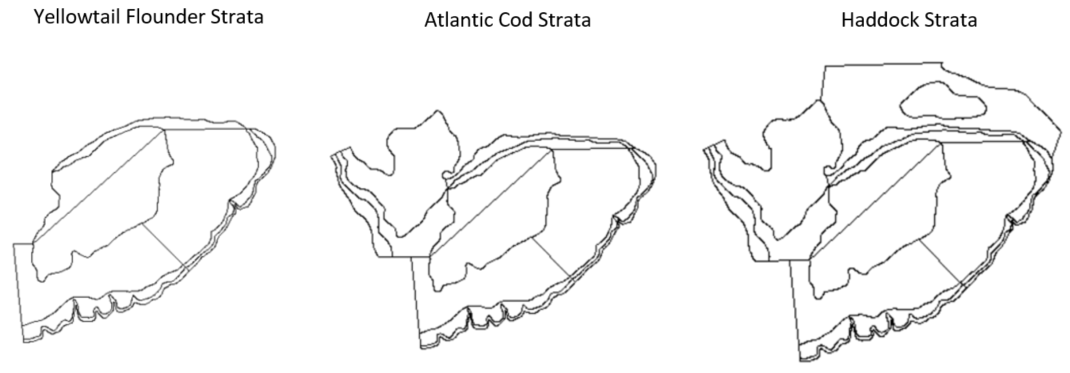
\includegraphics[width=0.95\linewidth]{Images/Strata} 

}

\caption{Strata inhabited by each species in our population models.}\label{fig:strata-plot}
\end{figure}

\emph{Population Dynamics and Recruitment}

The time step for our models is one week. MFS uses a modified two-stage Deriso-Schnute delay difference equation that models the biomass in each cell in our study area {[}@dolder2020highly{]}. Individual terms in the formulation account for growth of mature adults, natural and fishing mortality, and the addition of new recruits. We chose to represent recruitment in the model using a Beverton-Holt formulation \textbf{cite}. Recruitment is a function of the adult biomass that existed in the previous year and is added to the population incrementally throughout each species' predefined spawning period. Parameter inputs were either obtained from the literature or chosen to produce desired model dynamics. A full list of parameters used in our model can be seen below in Tables \ref{paramsALL} and \ref{tab:paramsSCENARIOS}.

\emph{Movement}

The package was designed to generate theoretical habitat preferences using Gaussian Random Fields that combine with hypothetical temperature gradients to drive the probability of movement from cell \(I\) to cell \(J\) using the formulation

\begin{align}
Pr(C_{wk+1}=J|C_{wk}=I) = \frac{e^{-\lambda \cdot d_{I,J}}\cdot(Hab^2_{J,s} \cdot Tol_{J,s,wk})}{\sum^C_{c=1}e^{-\lambda \cdot d} \cdot (Hab^2_{c,s} \cdot Tol_{c,s,wk})},
\label{moveP}
\end{align}

where

\(e^{-\lambda \cdot d_{I,J}}\) accounts for distance between cells \(I\) and \(J\),

\(Hab^2_{J,s}\) is the static habitat value for species \(s\) in cell \(J\), and

\(Tol_{c,s,wk}\) is the value from normally distributed temperature tolerance for species \(s\) in cell \(c\) in week \(wk\).

Since we are modeling real species on the northeast continental shelf, we formulate the habitat and temperature components as follows.

\emph{Habitat Input}

Species-specific habitat preferences were derived using the \emph{lrren} tool from the R package \emph{envi} \textbf{cite} to create a niche model for each species. The \emph{lrren} tool estimates an ecological niche using the relative risk function by relating presence/absence data to two covariate predictors. We used bottom trawl point data from 2009-2021 as our presence/absence input by using a value of 0 for any tow that failed to catch the given species and weighting a successful catch by the biomass of the given tow \textbf{cite trawl data?}. Depth and mean sediment size were used as our covariate predictors \textbf{cite}. Since the values in \(Hab^2_{J,s}\) are required to be between 0 and 1, we transform the spatial estimates from \emph{lrren} to fall between these bounds. See Figure ??? for a visual representation of this process being applied to Cod. Figure \ref{fig:hab-plot} depicts habitat preferences \(Hab^2_{J,s}\) for each species.

\begin{figure}

{\centering 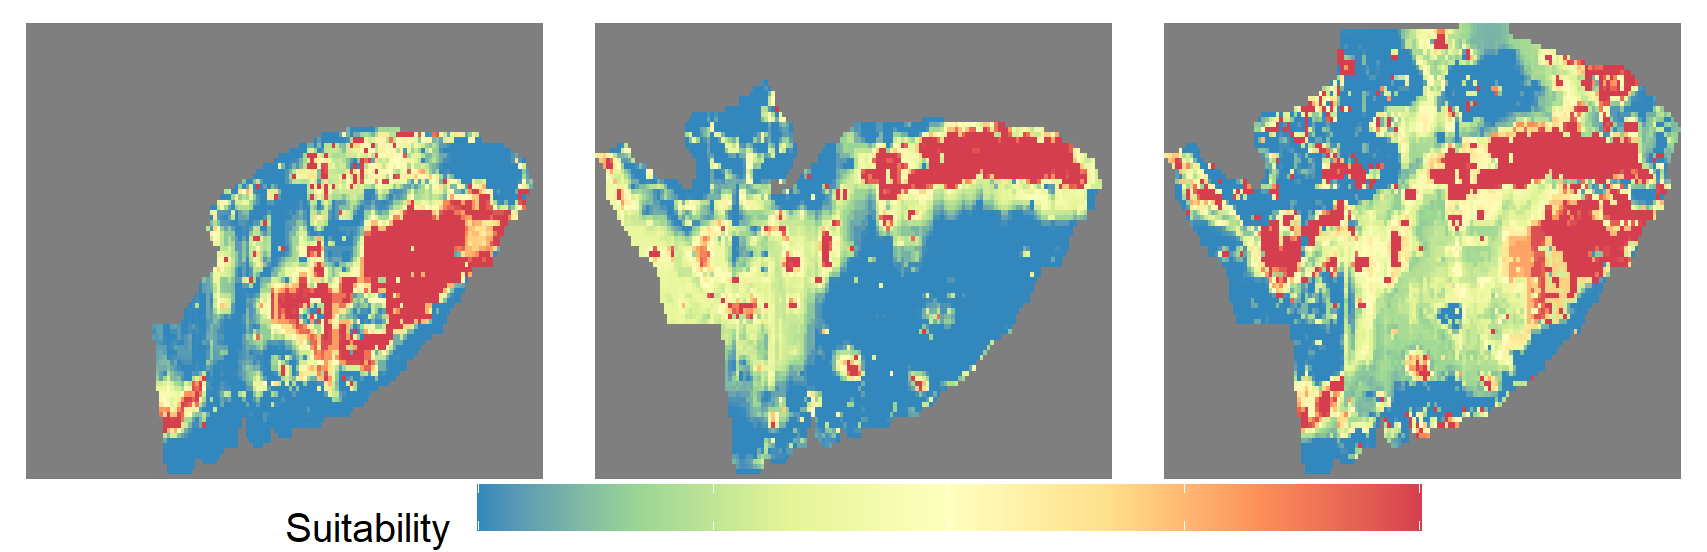
\includegraphics[width=0.95\linewidth]{Images/Habitat_3species} 

}

\caption{Static habitat preferences for each species in our population models (Yellotwtail, Cod, Haddock).}\label{fig:hab-plot}
\end{figure}

\emph{Temperature Input}

Each species is assumed to have normally distributed temperature preferences (\(N(\mu,\sigma)\)). We assume Yellowtail Flounder's preferences are \(N(8.75,4.25)\), while Haddock and Cod have preferences \(N(9,4)\). We chose these values by combining information in the literature with temperatures recorded in the bottom trawl survey. Weekly estimated temperature data for the region for 2012 was obtained from FVCOM \textbf{cite}. We chose 2012 because the data displayed an average temperature pattern that consistently oscillated between maximum and minimum temperature values. This data was also transform to create an oscillating pattern that increases 5 degrees Celsius on average over the duration of the simulation. \textbf{show images of temperature and/or and/or temp videos??? and/or average temperature oscillations?}

--Describe difference between increasing and constant temperature scenarios (images?)

In equation (1), \(Hab^2_{J,s}\) is constant for the duration of the simulation, while \(Tol_{c,s,wk}\) changes each week. Using a temperature gradient that repeats each year produces the same spatial preferences in a given week each year, which results in consistent spatial biomass patterns. Scenarios where the temperature increases over time creates spatial preferences that evolve as the water warms, which creates spatial biomass patterns that shift in a given week over the duration of the simulation.

-- Describe each scenario that is considered

We consider 20 year simulations under three population parameter scenarios for each of our three species- a scenario where parameters result in each population increasing over time, one where the populations are relatively constant over time, and a scenario where the parameter combination results in each population decreasing over time. Each of these three scenarios is paired with a temperature gradient that repeats as well as one that increasing roughly 5 degrees Celsius over the duration of the 20 year simulation. We therefore simulate a total of 6 scenarios. \textbf{show line plot of population for each?}

\emph{Simulating Bottom Trawl Survey and Population Indexing}

-Describe post hoc sampling process and how data is used

After each simulation is complete, we mimic the bottom trawl survey by conducting stratified random sampling in each inhabited strata twice each year. We sample in the same weeks that the Spring and Fall surveys take place and the number of the samples taken in each strata reflect true values. Most strata contain enough cells to sample a unique location in each survey over the duration of the simulation. For smaller strata we must repeat some sample locations. We then use the biomass collected from our samples in contemporary population indexing methods to estimate population trends. Knowing the true population values in our simulations allows us to compare the error calculated from each estimation method.

--Stratified mean vs VAST with and without covariates

We compare the yearly estimated of abundance obtained from the stratified mean to estimates obtained from the Vector-Autoregressive Spatio-temporal (VAST) model. The stratified mean is a typical survey-based approach that scales individual samples to the strata-level by considering the area of each strata, before scaling to the region-level based on the relative size of each strata. VAST is a spatio-temporal statistical framework that models both abundance (biomass) and probability of occurrence (presence/absence). If desired, VAST also allows users to include covariate data to better inform the model. Covariates can be static (eg. habitat preferences) or dynamics (eg. temperature). The stratified mean calculations are straightforward and quick, while VAST models require numerous user inputs and take on the order of hours to complete.

We follow the advice given in \textbf{cite Thorson 2019 Guidance\ldots{}} to build VAST models to estimate biomass on George's Bank using stratified mean samples from our model output. In addition to exploring different link functions and assumed distributions, our VAST model-building process included testing the impact of including spatial and/or spatio-temporal variation in our models, considering varying number of knots in our mesh, and testing different forms of temporal correlation. We also carried out the same process both including covariates in our model as well as running models without covariate information. We considered covaraites in the form of dyamic temperature values and/or static habitat values from our population model. When using covariates we ultimately decided to provide the most information to the model by including both covariates for both linear predictors. Since we know the true population values in our models we calculate the absolute error of each VAST estimate to compare between potential settings. Through this process, and in consultation with the VAST package creator, we determined setting that allowed VAST models to converge for all of our scenarios while also providing the lowest absolute error values. Settings for our VAST models can be seen in Table ???.

Our goal is to determine indexing approaches and settings that are robust to future environmental conditions and resulting spatial biomass patterns. An underlying assumption in all indexing methods that individual random samples combine to accurately represent true abudance by a) sampling all strata in which the population exists and b) low enough noise level in the samples to allow for a discernable pattern. This assumption can be questioned given enough noise in the sampling process \textbf{cite?} and/or shifting spatial preferences driven by climate change causing a population to move into a previously uninhabited strata. To simulate the impact of noise, indexing estimates after adding noise to our samples versus those using the true sampling values. To evaluate the effect of populations moving into new habitat, we compare indexing estimates using samples from all strata versus those that only include a subset of the full spatial domain for each species.

When combining population trends for each species, differing temperature scenarios, and sampling possibilities (noise, strata, covariates) there are a number of scenario combinations to consider. The columnbs in Table COMBOS show the possible choices that define each scenario.

Table COMBOS Each index estimate chooses one condition from each of the following columns. There are \(3*3*2*2*2*2=144\) VAST model combinations and \(3*3*2*2*2=72\) stratified mean estimates.

\begin{longtable}[]{@{}
  >{\raggedright\arraybackslash}p{(\columnwidth - 10\tabcolsep) * \real{0.16}}
  >{\raggedright\arraybackslash}p{(\columnwidth - 10\tabcolsep) * \real{0.16}}
  >{\raggedright\arraybackslash}p{(\columnwidth - 10\tabcolsep) * \real{0.16}}
  >{\raggedright\arraybackslash}p{(\columnwidth - 10\tabcolsep) * \real{0.16}}
  >{\raggedright\arraybackslash}p{(\columnwidth - 10\tabcolsep) * \real{0.16}}
  >{\raggedright\arraybackslash}p{(\columnwidth - 10\tabcolsep) * \real{0.21}}@{}}
\toprule
\begin{minipage}[b]{\linewidth}\raggedright
Species
\end{minipage} & \begin{minipage}[b]{\linewidth}\raggedright
Population Trend
\end{minipage} & \begin{minipage}[b]{\linewidth}\raggedright
Temperature Scenario
\end{minipage} & \begin{minipage}[b]{\linewidth}\raggedright
Strata Included
\end{minipage} & \begin{minipage}[b]{\linewidth}\raggedright
Noise in Data
\end{minipage} & \begin{minipage}[b]{\linewidth}\raggedright
Covariates (VAST only)
\end{minipage} \\
\midrule
\endhead
Yellowtail & Increasing & Repeating & All strata & No Noise & No Covariates \\
Cod & Constant & Increasing 5\(^{\circ}\) & Subset & Yes Noise & Temp + Habitat \\
Haddock & Decreasing & & & & \\
\bottomrule
\end{longtable}

\section{Results}

\begin{table}

\caption{\label{tab:unnamed-chunk-1}Yellowtail error results}
\centering
\begin{tabular}[t]{l|l|l|l|l|l|l|l|l|l|l|l}
\hline
X & X.1 & X.2 & X.3 & X.4 & Constant.Population & X.5 & Increasing.Population & X.6 & Decreasing.Population & X.7 & X.8\\
\hline
Temp & Covariate & Strata & Noise & season & Stratified Mean & VAST Estimate & Stratified Mean & VAST Estimate & Stratified Mean & VAST Estimate & \\
\hline
const & no cov & all & no & spring & 0.21 & 0.11 & 0.16 & 0.13 & 0.23 & 0.08 & \\
\hline
const & no cov & all & yes & spring & 0.25 & 0.16 & 0.22 & 0.21 & 0.27 & 0.11 & \\
\hline
const & w/ cov & all & no & spring & 0.21 & 0.07 & 0.16 & 0.06 & 0.23 & 0.06 & \\
\hline
const & w/ cov & all & yes & spring & 0.25 & 0.08 & 0.22 & 0.07 & 0.27 & 0.07 & \\
\hline
const & no cov & all & no & fall & 0.32 & 0.68 & 0.34 & 0.36 & 0.41 & 0.81 & \\
\hline
const & no cov & all & yes & fall & 0.31 & 0.77 & 0.46 & 0.44 & 0.44 & 1.09 & \\
\hline
const & w/ cov & all & no & fall & 0.32 & 0.08 & 0.34 & 0.08 & 0.41 & 0.08 & \\
\hline
const & w/ cov & all & yes & fall & 0.31 & 0.11 & 0.46 & 0.17 & 0.44 & 0.18 & \\
\hline
const & no cov & reduced & no & spring & 0.27 & 0.19 & 0.2 & 0.15 & 0.25 & 0.19 & \\
\hline
const & no cov & reduced & yes & spring & 0.26 & 0.15 & 0.22 & 0.11 & 0.3 & 0.16 & \\
\hline
const & w/ cov & reduced & no & spring & 0.27 & 0.19 & 0.2 & 0.17 & 0.25 & 0.19 & \\
\hline
const & w/ cov & reduced & yes & spring & 0.26 & 0.14 & 0.22 & 0.13 & 0.3 & 0.16 & \\
\hline
const & no cov & reduced & no & fall & 0.47 & 0.25 & 0.41 & 0.11 & 0.55 & 0.24 & \\
\hline
const & no cov & reduced & yes & fall & 0.49 & 0.36 & 0.46 & 0.21 & 0.53 & 0.36 & adding cov made worse\\
\hline
const & w/ cov & reduced & no & fall & 0.47 & 0.19 & 0.41 & 0.22 & 0.55 & 0.23 & \\
\hline
const & w/ cov & reduced & yes & fall & 0.49 & 0.17 & 0.46 & 0.19 & 0.53 & 0.24 & \\
\hline
increasing & no cov & all & no & spring & 0.28 & 0.11 & 0.32 & 0.13 & 0.22 & 0.15 & \\
\hline
increasing & no cov & all & yes & spring & 0.28 & 0.15 & 0.34 & 0.16 & 0.26 & 0.17 & cov really helped\\
\hline
increasing & w/ cov & all & no & spring & 0.28 & 0.06 & 0.32 & 0.07 & 0.22 & 0.07 & \\
\hline
increasing & w/ cov & all & yes & spring & 0.28 & 0.12 & 0.34 & 0.1 & 0.26 & 0.1 & \\
\hline
increasing & no cov & all & no & fall & 0.51 & 1.26 & 0.3 & 0.66 & 0.28 & 1.06 & \\
\hline
increasing & no cov & all & yes & fall & 0.5 & 1.38 & 0.39 & 0.71 & 0.25 & 1.1 & \\
\hline
increasing & w/ cov & all & no & fall & 0.51 & 0.23 & 0.3 & 0.21 & 0.28 & 0.15 & cov good, why no cov so bad???\\
\hline
increasing & w/ cov & all & yes & fall & 0.5 & 0.28 & 0.3 & 0.37 & 0.25 & 0.2 & \\
\hline
increasing & no cov & reduced & no & spring & 0.31 & 0.17 & 0.4 & 0.33 & 0.32 & 0.14 & \\
\hline
increasing & no cov & reduced & yes & spring & 0.29 & 0.19 & 0.41 & 0.26 & 0.29 & 0.15 & \\
\hline
increasing & w/ cov & reduced & no & spring & 0.31 & 0.17 & 0.4 & 0.3 & 0.32 & 0.22 & \\
\hline
increasing & w/ cov & reduced & yes & spring & 0.29 & 0.15 & 0.41 & 0.25 & 0.29 & 0.21 & \\
\hline
increasing & no cov & reduced & no & fall & 0.64 & 0.75 & 0.7 & 0.49 & 0.54 & 0.6 & \\
\hline
increasing & no cov & reduced & yes & fall & 0.66 & 0.89 & 0.69 & 0.48 & 0.53 & 0.62 & cov didnt do much\\
\hline
increasing & w/ cov & reduced & no & fall & 0.64 & 0.2 & 0.7 & 0.53 & 0.54 & 0.31 & \\
\hline
increasing & w/ cov & reduced & yes & fall & 0.66 & 0.13 & 0.69 & 0.5 & 0.53 & 0.32 & \\
\hline
\end{tabular}
\end{table}

\begin{table}

\caption{\label{tab:unnamed-chunk-1}Cod error results}
\centering
\begin{tabular}[t]{l|l|l|l|r|r|r|l|l}
\hline
Temp & Strata & Noise & season & VAST.No.Cov & VAST.w..Cov & Stratified.Mean & X & X.1\\
\hline
const & all & no & spring & 0.11 & 0.12 & 0.36 & NA & \\
\hline
const & all & yes & spring & 0.12 & 0.15 & 0.35 & NA & Cod\\
\hline
const & all & no & fall & 0.19 & 0.05 & 0.49 & NA & Decreasing Population\\
\hline
const & all & yes & fall & 0.30 & 0.23 & 0.41 & NA & \\
\hline
const & reduced & no & spring & 0.17 & 0.24 & 0.41 & NA & \\
\hline
const & reduced & yes & spring & 0.20 & 0.23 & 0.46 & NA & \\
\hline
const & reduced & no & fall & 0.21 & 0.33 & 0.60 & NA & \\
\hline
const & reduced & yes & fall & 0.18 & 0.31 & 0.58 & NA & \\
\hline
increasing & all & no & spring & 0.12 & 0.15 & 0.25 & NA & \\
\hline
increasing & all & yes & spring & 0.19 & 0.19 & 0.27 & NA & \\
\hline
increasing & all & no & fall & 0.76 & 0.13 & 0.45 & NA & \\
\hline
increasing & all & yes & fall & 0.89 & 0.33 & 0.44 & NA & \\
\hline
increasing & reduced & no & spring & 0.14 & 0.22 & 0.32 & NA & \\
\hline
increasing & reduced & yes & spring & 0.15 & 0.21 & 0.29 & NA & \\
\hline
increasing & reduced & no & fall & 0.60 & 0.31 & 0.54 & NA & \\
\hline
increasing & reduced & yes & fall & 0.62 & 0.32 & 0.53 & NA & \\
\hline
\end{tabular}
\end{table}

\begin{table}

\caption{\label{tab:unnamed-chunk-1}Haddock error results}
\centering
\begin{tabular}[t]{l|l|l|l|r|r|r|l|l}
\hline
Temp & Strata & Noise & season & VAST.No.Cov & VAST.w..Cov & Stratified.Mean & X & X.1\\
\hline
const & all & no & spring & 0.49 & 0.18 & 0.18 & NA & \\
\hline
const & all & yes & spring & 0.73 & 0.43 & 0.21 & NA & Haddock\\
\hline
const & all & no & fall & 0.28 & 0.05 & 0.26 & NA & Increasing Population\\
\hline
const & all & yes & fall & 0.41 & 0.06 & 0.27 & NA & \\
\hline
const & reduced & no & spring & 0.34 & 0.35 & 0.45 & NA & \\
\hline
const & reduced & yes & spring & 0.30 & 0.33 & 0.46 & NA & \\
\hline
const & reduced & no & fall & 0.36 & 0.48 & 0.54 & NA & \\
\hline
const & reduced & yes & fall & 0.33 & 0.46 & 0.52 & NA & \\
\hline
increasing & all & no & spring & 0.25 & 0.05 & 0.26 & NA & \\
\hline
increasing & all & yes & spring & 0.30 & 0.06 & 0.31 & NA & \\
\hline
increasing & all & no & fall & 0.89 & 0.23 & 0.40 & NA & \\
\hline
increasing & all & yes & fall & 1.04 & 0.35 & 0.42 & NA & \\
\hline
increasing & reduced & no & spring & 0.32 & 0.40 & 0.44 & NA & \\
\hline
increasing & reduced & yes & spring & 0.38 & 0.37 & 0.37 & NA & \\
\hline
increasing & reduced & no & fall & 0.44 & 0.64 & 0.72 & NA & \\
\hline
increasing & reduced & yes & fall & 0.42 & 0.62 & 0.70 & NA & \\
\hline
\end{tabular}
\end{table}

\hypertarget{discussion}{%
\subsection{Discussion}\label{discussion}}

A range of data-limited methods for setting catch advice were evaluated for stocks where assessment models may be rejected due to strong, positive retrospective patterns. A method was considered to perform well if it limited overfishing without resulting in light exploitation rates (\(F << F_{MSY}\)), thereby allowing depleted stocks to recover to \(SSB_{MSY}\) (or for healthy stocks to remain there), and for high and stable catches (close to \(MSY\)).

Overall, none of the methods evaluated performed best across the scenarios exploring the different sources of the retrospective pattern (unreported catch or increasing \(M\)) and different levels of historical fishing intensity. A number of methods did perform well in many cases, however, while others performed consistently poorly, resulting in frequent and intense overfishing (\(F>>F_{MSY}\)). We performed simulations for a couple of scenarios with no source of retrospective patterns and found the expected result that all DLMs and the SCAA performed better (\(SSB\), \(F\), and catch were all closer to the \(MSY\) reference points) than when either source of retrospective patterns was present. Due to the focus of this study, we did not examine the no retrospective source in detail and do not comment on it further.

Currently, in the Northeast U.S., if an assessment model is rejected due to a large rho value in \(SSB\), the catch advice from that model is ignored and some data-limited approach is used. However, the rho-adjusted SCAA model performed better than a number of the alternatives explored here. Therefore, there should not necessarily be an expectation that a data-limited method will perform better than the rejected assessment model. The SCAA only resulted in high exploitation rates (\(F >> F_{MSY}\)) when unreported catch was the source of the retrospective pattern and for the scenario where \(F=F_{MSY}\) at the end of the base period that left the stock in relatively good condition (\(SSB \sim SSB_{MSY}\)). In contrast, this method was particularly effective when the stock was depleted and there was unreported catch. When \(M\) was the source of the retrospective pattern, the rho-adjusted SCAA method typically resulted in light exploitation rates, on average. The light exploitation rates in these cases were likely driven by the combination of using a rho-adjustment, but also using the lower \(M\) from the beginning of the base period rather than the higher \(M\) that occurred during the feedback period. Using an \(M\) value that is too low in a stock assessment will typically bias estimates of biomass and reference points too low, resulting in catch advice that is below target levels {[}@Johnsonetal2014; @Puntetal2021M{]}. The consequences of using a value for \(M\) that is too low versus too high is also asymmetrical {[}@Johnsonetal2014{]}, with negative consequences being more severe when \(M\) is assumed too high than low, and the results here are consistent with these previous conclusions.

The methods that adjusted recent average catches based on trends in the survey (Ismooth and Islope) performed well overall in terms of catch, stock status, and variation in catch. The method using the expanded survey biomass with the recent exploitation rate (ES-Frecent) also performed well and similarly to Ismooth. The performance of these methods was also generally robust among scenarios, with the exception of when there were unreported catches and the stock was depleted (see below). The generally positive performance of these methods was consistent with @Hilbornetal2002 and @CoxKronlund2008, both of which evaluated a variant of a ``hold-steady'' DLM. In the case of @Hilbornetal2002, the ``hold-steady'' DLM policy was designed to adjust catches in order to keep rockfish (\emph{Sebastes spp.}) populations at recently observed index levels, and did so by functioning as a constant escapement harvest control rule where target catches were set to zero below some pre-specified index level. In the variant used by @CoxKronlund2008, catches were adjusted to maintain a sablefish (\emph{Anoplopoma fimbria}) population at a pre-specified index level thought to be sustainable and desirable in terms of meeting fishery objectives (e.g., high catch), but never permitted target catches of zero and so functioned as a constant exploitation rate control rule. The ``hold-steady'' DLM of @CoxKronlund2008 performed similarly in terms of catch, stock depletion, and variation in catch, as a constant exploitation rate policy where target catch was specified as the product of desired exploitation rate and an estimate of biomass from a SCAA model. This result was robust to uncertainty in initial stock status and steepness {[}@CoxKronlund2008{]}. The SCAA model was always correctly specified (i.e., expected to produce unbiased estimates on average), however, and no comparison to the results of this research in the presence of retrospective patterns is possible {[}@CoxKronlund2008{]}. The ``hold-steady'' policy of @Hilbornetal2002 performed similarly to or better in terms of catch and stock status than other harvest control rules that relied on assessment estimates of biomass (i.e., 40:10 and constant \emph{F}). The performance of the ``hold-steady'' DLM was also more robust to uncertainty in steepness and to the presence of unreported catch {[}@Hilbornetal2002{]}. The performance of the two harvest policies that relied on assessment estimates of biomass (i.e., constant exploitation rate and a ``40:10'' biomass-based policy) also degraded when the estimates of biomass were biased, which is an issue that does not effect the ``hold-steady'' DLM {[}@Hilbornetal2002{]}. The bias in the assessment estimates considered in @Hilbornetal2002 were not necessarily induced by a retrospective pattern, however, and no consideration of making a rho-adjustment was possible in that study.

The Ismooth method is currently used to set catches for Georges Bank cod {[}@nefsc19{]} and red hake (\emph{Urophycis chuss}; @nefsc20). Variations of the ES-Frecent have been used for witch flounder and Georges Bank yellowtail flounder. While the findings here generally support the continued use of the Ismooth and ES-Frecent methods, they may not be well suited for depleted stocks where unreported catches are believed to be an issue. The Ismooth, Islope, and ES-Frecent DLMs produced high \(Fs\) and limited stock recovery with unreported catches and when the stock was depleted. While @Hilbornetal2002 and @CoxKronlund2008 did not reach the same conclusion about the ``hold-steady'' DLM, those studies did not consider initial levels of depletion as low as in this study. These results highlight the importance of accurate catch reporting, as unreported catch can create a negative feedback loop with perpetually high \(Fs\) being produced by a management system that seemingly should result in sustainable catch advice.

Three methods were consistently risk-averse across scenarios, limiting the frequency and magnitude of overfishing and resulting in high stock biomass. These methods were the two catch curve options (CC-FM and CC-FSPR) and DynLin. The catch curve methods produced a wider range of average catches across scenarios, and also had greater interannual variability in catches compared to DynLin. While the lower exploitation rates from these approaches may be undesirable due to forgone yield, there may be circumstances where they are preferred. For example, for stocks that are believed to be heavily depleted, low exploitation rates would allow for a more rapid recovery.

A number of methods performed poorly, particularly when catches were unreported. These methods include three of the expanded survey biomass approaches (ES-Fstable, ES-FM, ES-FSPR), AIM, and Skate. The AIM model has been widely used across stocks in the region {[}@nefsc02a; @nefsc05; @nefsc08{]}, although there is a decreasing trend in its use across model resistant stocks {[}@nefsc19{]}. The findings here suggest that alternative approaches should be considered in cases where AIM is still used and there is concern over unreported catches. The Skate method is used to manage the skate complex in the Northeast U.S. (a group of seven co-managed species). Interestingly, six of the seven species are considered in good condition with high survey biomass indices in recent years {[}@nefmc20{]}. That the Skate method performed poorly in our analysis but performs well for the skate complex illustrates how the performance of methods in this analysis may be sensitive to the scenarios and species life history considered. As may be the case for the Skate method, the performance of some methods may depend on the condition of the stock when the method is first applied, and less so on life-history. Therefore, care is needed when trying to generalize these results across stocks that may have different life histories, exploitation histories, and without unreported catches or increases in \(M\).

In addition to the analytical differences among the thirteen DLMs, most of the DLMs and control rules had multiple options that could be adjusted to make them more or less risk averse. DynLin had a large number of user defined decision points. Given the large range of options already explored in the study, one suite of options was selected for each DLM-control rule and kept constant for all simulations. Further studies could explore the different options within an individual DLM to understand how they might affect performance.

Many other data-limited methods exist for setting catch advice that were not included in this evaluation, and they vary widely in complexity, data inputs, and assumptions required {[}e.g., @carruthers2018dlm{]}. Length based methods were not evaluated to keep the overall number of methods tractable, and due to the availability of age based information in the region. Methods that require only catch data or snap shots of survey data were not considered due to the availability of the relatively long and contiguous Northeast Fisheries Science Center's spring and fall, coastwide bottom trawl surveys, and the fact that ``catch only'' methods have been shown to perform poorly {[}e.g., @carruthers2014eval{]}. Complete catch histories are not available for stocks in the region (i.e., from the inception of fishing). Consequently, methods that required complete catch histories or required assumptions about relative depletion {[}e.g., DCAC in @maccall2009dca; DB-SRA in @dick2022dsra{]} were also omitted from consideration. The need for short run-times and the desire for methods that could be reviewed quickly prevented the use of modern state-space production models such as SPiCT {[}@pedersen2017spict{]} and JABBA {[}@winker2018jabba{]}.

The SCAA was confronted with inconsistent data in this study, while the DLMs typically used only a single source of data and thus did not encounter inconsistencies. A recent examination of the data used in assessments in this region similarly found inconsistencies in data streams even before modeling. @wiedenmann2022strange found a negative relationship between relative F (catch/survey) and survey Z for stocks with strong retrospective patterns but the expected positive relationship for stocks without a retrospective pattern. It is exactly this sort of tension that creates retrospective patterns in integrated models, but is not found in DLMs that only use one type of data.

Despite conducting hundreds of thousands of simulations, there are still limitations to our study. We only examined one life history representative of groundfish in the region. We acknowledge that best practice is to select a DLM for a specific life history and fishery condition {[}e.g., @fischer2020dlm{]}. As is typically the case with large simulation studies, we were not able to tune any of the DLMs or the SCAA in any given realization, which would occur in practice for an actual stock assessment. We also examined only scenarios that started with Mohn's rho values near 0.5 for spawning stock biomass. This is a strong retrospective pattern, but some stocks in the region have even stronger retrospectives. Performance of the DLMs and SCAA would be expected to degrade with stronger retrospectives, but by how much is still an open area for research. Similarly, sources of retrospective patterns that create different relationships between the true values and estimated values should also be explored {[}see @deroba2014retro{]}. To make the results interpretable, we only examined a single source for the retrospective pattern at a time. In reality, there may be more than one factor leading to an observed retrospective pattern. How the multiple sources would interact to influence performance is another topic for future research. Development of harvest control rules specifically for situations where retrospective patterns are found in age-based assessments would also be beneficial. The large number of scenarios examined and the large number of realizations gives us confidence that our results are meaningful in general, but that the performance of any of the DLMs may differ in actual practice.

An interesting finding of this study is the linear versus diffuse patterns between \(SSB\) and catch across methods. These patterns have implications for the trade-offs among methods, with linear relationships resulting in more consistent exploitation rates across stock sizes. Therefore, these methods have higher certainty of a given catch at a given stock size. However, they also tended to result in lower stock sizes, on average, across methods. The more diffuse relationships resulted in more variable exploitation rates across stock sizes, with some situations where the population biomass was quite high but the catch was low (relative to MSY), resulting in a very low \(F\). The reasons behind these different patterns remain unclear, and future work to explore these patterns is warranted.

One of the reasons for the difference in performance between the catch and natural mortality retrospective sources was how the reference points were calculated. In all cases, the initial conditions, including the natural mortality rate, were used to compute the reference points. This decision was made based on the fact that the increase in natural mortality was assumed to be unknown in the simulations. If the increase in natural mortality was known, the age-structured assessments would have accounted for it, different reference points might have been computed {[}@legault2016increaseM{]} and there may not have been a retrospective pattern at all {[}@legault2020rose{]}, and no need to consider alternative DLMs. The reference points for the increased \(M\) scenarios would have been different if they were computed using the values from the final year of the base period, but the overall conclusions regarding the different DLMs would not change as this just results in a rescaling of the axis. These results are not shown to reduce confusion regarding the simulations.

Closed-loop simulation is a common tool for examining performance of catch advice from various stock assessment approaches in a feedback setting. It is often used as part of a full management strategy evaluation when working with stakeholders to develop management regulations that make trade offs between near term and long term catches, risk to the fish population, and mixed-fleet allocations {[}@carruthers2016simpleMPs; @goethel2019mse; @harlyan2019hcr{]}. We did not conduct a full management strategy evaluation with stakeholder input {[}@goethel2019stakeholder{]}, but see that as a fruitful next step that could build on the conclusions from our closed-loop work. Using a generic groundfish life-history and monitoring standard performance metrics related to stock status and catch stability, we were able to cull the herd of potential DLMs and we would not carry the consistent poor performers forward for further study. The wide range of expertise reflected in the authorship was by design so that the simulation specifications and performance metrics were broadly useful. Before undertaking a full management strategy evaluation and engaging regional stakeholders, we would want to select a specific stock and jointly identify specific management regulations to be tested {[}@deroba2019dream{]}. Results of this work have been presented to both local fishery management councils, with generally positive feedback about the utility of the conclusions for identifying appropriate model approaches when an SCAA is rejected. Our work was similar to all other closed-loop simulations in that it was designed to address a specific situation, including much recent work comparing the performance of data-limited and data rich assessment approaches {[}e.g., @fulton2016datarich; @sagarese2019dlm; @bouch2020datapoor; @li2022dlm{]}.

This study is a first attempt to identify suitable methods for setting catch advice when stock assessment models are rejected due to large, positive retrospective patterns. Although no single method performed best across scenarios, a number of generally suitable and unsuitable methods were identified under specific conditions. The results of this work can help scientists and managers select a subset of possible options for consideration to set catch advice when assessment models are rejected. The approach developed here can, and should be expanded to consider other cases not explored here, as performance of individual methods are very likely case-dependent.

\hypertarget{acknowledgements}{%
\subsection{Acknowledgements}\label{acknowledgements}}

We thank the Index-Based Methods and Control Rules Research Track review panel of Paul Rago (chair), Yong Chen, Robin Cook, and Paul Medley for feedback on preliminary results, three anonymous reviewers and the associate editor for reviewing an earlier version of this work. The scientific results and conclusions, as well as any views or opinions expressed herein, are those of the authors and do not necessarily reflect those of NOAA or the Department of Commerce.

\hypertarget{data-and-code-availability}{%
\subsection{Data and Code Availability}\label{data-and-code-availability}}

All data and code used in this work are available at \url{https://github.com/cmlegault/IBMWG}.

\hypertarget{references}{%
\subsection{References}\label{references}}

\hypertarget{refs}{}
\begin{CSLReferences}{0}{0}
\end{CSLReferences}

\pagebreak

\hypertarget{tables}{%
\subsection{Tables}\label{tables}}

\pagebreak

Table 1. Parameters used in all population models.

\begin{longtable}[]{@{}lllllll@{}}
\toprule
Parameter & Description & Unit & Yellowtail & Cod & Haddock & Source \\
\midrule
\endhead
\(\rho\) & Ford's growth coefficient & wk\(^{-1}\) & 4.48 & 4.43 & 4.49 & \\
\(M\) & Natural Mortality & wk\(^{-1}\) & 0.2064 & 0.2728 & 0.3340 & \\
\(W_R\) & Weight of fully recruited fish & kg & 0.39 & 2.95 & 1.12 & \\
\(W_{R-1}\) & Weight of pre-recruit fish & kg & 0.13 & 0.39 & 0.19 & \\
\(\sigma^2\) & Variance in recruited fish & kg\(^2\) & 0.55 & 0.55 & 0.55 & \\
\(\lambda\) & Decay rate for movement & - & 0.7 & 0.7 & 0.7 & \\
\(Spwn_s\) & Spawning weeks for species \(s\) & wk & 9-12 & 8-13 & 11-14 & \\
\(Rec_s\) & Recruitment weeks for species \(s\) & wk & 9-12 & 8-13 & 11-14 & \\
\bottomrule
\end{longtable}

\begin{table}
 
 \caption{\label{tab:paramsALL2}Parameters used in all population models.}
 \centering
 \fontsize{10}{12}\selectfont
 \begin{tabular}[t]{lllllll}
 \toprule
 Parameter & Description & Unit & Yellowtail & Cod & Haddock & Source\\
 \midrule
 <U+03C1> & Ford's growth coefficient & 1/wk & 4.48 & 4.43 & 4.49 & NA\\
 M & Natural mortality & 1/wk & 0.2064 & 0.2728 & 0.334 & NA\\
 W1 & Weight of fully recruited fish & kg & 0.39 & 2.95 & 1.12 & NA\\
 W2 & Weight of pre-recruit fish & kg & 0.13 & 0.39 & 0.19 & NA\\
 sigma & Variance in recruited fish & kg*kg & 0.55 & 0.55 & 0.55 & NA\\
 \addlinespace
 lambda & Decay rate for movement & - & 0.7 & 0.7 & 0.7 & NA\\
 spwn & Spawning weeks for species s & wks & 9-12 & 8-13 & 11-14 & NA\\
 rec & Recruitment weeks for species s & wks & 9-12 & 8-13 & 11-14 & NA\\
 \bottomrule
 \end{tabular}
 \end{table}

\begin{table}

\caption{\label{tab:paramsSCENARIOS}Parameters used in population models for each scenario.}
\centering
\fontsize{10}{12}\selectfont
\begin{tabular}[t]{llllll}
\toprule
Parameter & Description & Unit & Yellowtail & Cod & Haddock\\
\midrule
\addlinespace[0.3em]
\multicolumn{1}{l}{\textbf{Constant Population}}\\
\hspace{1em}M+F & Adjusted Mortality (Natural + Fishing) & 1/wk & 0.764 & 0.83 & 0.309\\
\hspace{1em}P0 & Initial Biomass & kg & 3190 & 21500 & \vphantom{1} 180000\\
\hspace{1em}a & Max recruitment rate & kg & 30400 & 27900 & 73600\\
\hspace{1em}ß & Recruitment half saturation value & kg & 4300 & 10500 & 40500\\
\addlinespace[0.3em]
\multicolumn{1}{l}{\textbf{Decreasing Population}}\\
\hspace{1em}M+F & Adjusted Mortality (Natural + Fishing) & 1/wk & 0.764 & 0.623 & 0.334\\
\hspace{1em}P0 & Initial Biomass & kg & 50000 & 21500 & 180000\\
\hspace{1em}a & Max recruitment rate & kg & 1.07e+12 & 3.89e+08 & 4.97e+08\\
\hspace{1em}ß & Recruitment half saturation value & kg & 2.3e+12 & 9.8e+08 & 2.08e+09\\
\addlinespace[0.3em]
\multicolumn{1}{l}{\textbf{Increasing Population}}\\
\hspace{1em}M+F & Adjusted Mortality (Natural + Fishing) & 1/wk & 0.564 & 0.372 & 0.134\\
\hspace{1em}P0 & Initial Biomass & kg & 3190 & 21500 & 180000\\
\hspace{1em}a & Max recruitment rate & kg & 40000 & 45000 & 1e+05\\
\hspace{1em}ß & Recruitment half saturation value & kg & 43000 & 62800 & 405000\\
\bottomrule
\end{tabular}
\end{table}

Table XX. Parameters used in all VAST models.

\begin{longtable}[]{@{}
  >{\raggedright\arraybackslash}p{(\columnwidth - 4\tabcolsep) * \real{0.13}}
  >{\raggedright\arraybackslash}p{(\columnwidth - 4\tabcolsep) * \real{0.53}}
  >{\raggedright\arraybackslash}p{(\columnwidth - 4\tabcolsep) * \real{0.33}}@{}}
\toprule
\begin{minipage}[b]{\linewidth}\raggedright
Parameter
\end{minipage} & \begin{minipage}[b]{\linewidth}\raggedright
Description
\end{minipage} & \begin{minipage}[b]{\linewidth}\raggedright
Input/Value
\end{minipage} \\
\midrule
\endhead
\emph{ObsModel} & Link function and assumed distribution & c(10,2) \\
FieldCOnfig & Specified spatial and/or spatio-temporal variation in predictors & c(Omega1=0, Epsilon1=0, Omega2=1, Epsilon2=1) \\
RhoConfig & Specifying whether intercepts or spatio-temporal variation is structured among time intervals & c(Beta1=3, Beta2=3, Epsilon1=0, Epsilon2=4) \\
X1\_formula & Right-sided formula affecting the 1st linear predictor & X1\_formula = \textasciitilde{} poly(Temp, degree=2 ) \\
X2\_formula & Right-sided formula affecting the 2nd linear predictor & X2\_formula = \textasciitilde{} poly(Temp, degree=2 ) + poly(Habitat, degree=2 ) \\
\bottomrule
\end{longtable}

\end{document}
